\documentclass[procedia]{easychair}
\usepackage{url}
\usepackage[flushleft]{threeparttable}
\hyphenation{resour-ces}
\hyphenation{approac-hes}
\hyphenation{har-der}
\hyphenation{spe-cifically}
\makeatletter
\def\@copyrightspace{\relax}
\makeatother

\usepackage{comment}
\usepackage{wrapfig}
\excludecomment{TM}

\title{An Invariant Framework for Conducting Reproducible Computational Science}

\titlerunning{An invariant framework for conducting reproducible computational science}

\author{
	Haiyan Meng\inst{2}
\and Rupa Kommineni\inst{1}
\and Quan Pham\inst{1} \\
\and Robert Gardner\inst{1}
\and Tanu Malik\inst{1}
\and
	Douglas Thain\inst{2}
}
\institute{
	Computation Institute,
	University of Chicago,
	Chicago, Illinois, USA \\
	\email{rupa, quanpt, rwg, tanum@uchicago.edu}
\and
	Department of Computer Science and Engineering,
	University of Notre Dame,
	Notre Dame, Indiana, USA \\
	\email{hmeng, dthain@nd.edu}
}

%  \authorrunning{} has to be set for the shorter version of the authors' names;
% otherwise a warning will be rendered in the running heads. When processed by
% EasyChair, this command is mandatory: a document without \authorrunning
% will be rejected by EasyChair

\authorrunning{Meng et al.}

\begin{document}

\maketitle

\keywords{Preservation framework, reproducible research, virtualization, container}

\begin{abstract}
\it Computational reproducibility depends on the ability to not only isolate necessary and sufficient computational artifacts but also to preserve those artifacts for later re-execution. Both isolation and preservation present challenges in large part due to the complexity of existing software and systems as well as the implicit dependencies, resource distribution, and shifting compatibility of systems that result over time---all of which conspire to break the reproducibility of an application. Sandboxing is a technique that has been used extensively in OS environments in order to isolate computational artifacts. Several tools were proposed recently that employ sandboxing as a mechanism to ensure reproducibility. However, none of these tools preserve the sandboxed application for re-distribution to a larger scientific community—aspects that are equally crucial for ensuring reproducibility as sandboxing itself. In this paper, we describe a framework of combined sandboxing and preservation, which is not only efficient and invariant, but also practical for large-scale reproducibility. We present case studies of complex high-energy physics applications and show how the framework can be useful for sandboxing, preserving, and distributing applications. We report on the completeness, performance, and efficiency of the framework, and suggest possible standardization approaches. 

\end{abstract}

\vspace{-10pt}
\section{Introduction}

Reproducibility is a cornerstone of the scientific method~\cite{borgman2012data}. 
Its ability to advance science underscores its importance---reproducing by verifying and validating a scientific result leads to improved understanding, thus increasing possibilities of reusing or extending the result. 
Ensuring the reproducibility of a scientific result, however, often entails detailed documentation and specification of the involved scientific method. Historically, text and proofs in a publication have achieved this end. 
As computation pervades the sciences and transforms the scientific method, simple text and static images are no longer sufficient. 
In particular, apart from textual (and numeric) descriptions describing the result, a reproducible result must also include several computational artifacts, such as software, data, environment variables, platform dependencies and the state of computation that are involved in the adopted scientific method \cite{Sole}.  

Virtualization has emerged as a promising technology to reproduce computational scientific results.  One such approach is to conduct the entire computation relating to a scientific result within a virtual machine image, and then preserve and share the resulting image. This way "VMI"s become an authoritative, encapsulated, and executable record of the computation, especially computations whose results are destined for publication and/or re-use.  Virtual machine images, like files, can then be shared \cite{Lampoudi}. 
The resulting image, however, may be too large to share or distribute widely. An alternative light-weight form of virtualization is to encapsulate only the application software along with all its necessary dependencies into a self-contained package. The encapsulation is achieved by operating system-level sandboxing techniques that interpose application system calls and copy the necessary dependencies (data, libraries, code, etc.) into a package, making it lighter weight than a VMI~\cite{guo2011cde}. Yet, the package is not longer an executable record of the computation and still requires an accompanying operating system for execution. 

While both approaches provide mechanisms for encapsulating the computations associated with a scientific result, neither form of virtualization provides any guarantee that the included pieces of software will indeed reproduce the associated scientific result. In general, in the absence of reproducible policy guidelines, such guarantees can be difficult to provide. Preserving the encapsulated computations in such a way that they are always reproducible will improve upon the guarantees. A preservation mechanism can increase the ease of image or package installation, alter dependencies implicit to computation as software components evolve or become deprecated, and provide mechanisms for documentation that make computations easy to understand after the fact.

%Since reproducibility includes documentation, virtualization approaches in their current form only make it easy to capture the computations. Preserving the computations so that they are easy to understand, install, or alter implicit dependencies that are part of computation is not effectively addressed, especially as dependencies and software components evolve or become deprecated. 

The two approaches that address the preservation challenge are as follows: one, the introduction of tools that help document dependencies and provide software attribution within VMIs or packages; and two, the use of software delivery mechanisms such as centralized package management, Linux containers, and the more recent Docker framework. We examined the first approach previously in \cite{SoftProv}. 
In this paper we examine the second approach.  We consider in particular the lightweight virtualization because we believe together with more standardized software delivery mechanisms, the two combined can address the reproducibility challenge for a wide variety of scientific researchers. A package created by those lightweight approaches encapsulates all the necessary dependencies of an application, and can be used to repeat the application through different sandbox mechanisms, including Parrot
%In particular, we consider the light-weight virtualization approaches, because, we believe that a combination of light-weight approaches with more standardized software delivery mechanisms can lead to addressing the reproducibility challenge for a wide variety of scientific researchers.  
%A package created by those light-weight approaches encapsulates all the necessary dependencies of an application, and can be used to repeat the application through different sandbox mechanisms, including Parrot
~\cite{thain2005parrot}, CDE~\cite{guo2011cde}, PTU~\cite{PTU}, chroot, and Docker~\cite{boettiger2015introduction}. 

Of course our solution represents only one way to preserve applications. Broadly, two different approaches to preserve applications have been adopted: force cleanliness or measure the mess. The former forces users to specify the execution environment for an application in a well-organized way. The latter causes end users to construct the environment as desired, and the complexity of the environment is measured in terms of its dependencies. Our objective here is to measure the mess as-is and then preserve it over time.

%We do not claim our solution is the only way to preserve applications. Broadly, there are two different approaches to preserve applications: force cleanliness or measure the mess. The first approach forces users to specify the execution environment for an application in a well organized way. In the latter one end users construct the environment as desired, and the complexity of the environment is measured in terms of its dependencies. 
%Our objective here is to measure the mess as-is and then preserve it over time.

To conduct a thorough examination, we consider real-world complex high energy physics (HEP) applications, independently developed by two groups, that must be reproduced so that the entire HEP community can benefit from the analysis. We describe challenges faced in reproducing the applications, and we consider the extent to which reproducibility requirements can be satisfied with lightweight virtualization approaches and software delivery mechanisms. We propose an invariant framework for computational reproducibility that combines lightweight virtualization with software delivery mechanisms for efficiently capturing, invariantly preserving, and practically deploying applications. We measure the performance overhead of lightweight virtualization and software delivery approaches, and show how the preserved packages can be distributed to allow reproduction and verification.
%To conduct a thorough examination, we consider real-world complex high energy physics (HEP) applications, independently developed by two groups, that must be reproduced so that the entire HEP community can benefit from the analysis. We describe challenges in reproducing the applications, and consider the extent to which reproducibility requirements can be satisfied with light-weight virtualization approaches and software delivery mechanisms. We propose an invariant framework for computational reproducibility that combines light-weight virtualization with software delivery mechanisms for efficiently capturing, invariantly preserving and practically deploying applications.
%We measure the performance overhead of  light-weight virtualization and software delivery approaches, and show the preserved packages can be distributed to allow reproduction and verification.


\vspace{-10pt}
\begin{figure}[t]
\centering
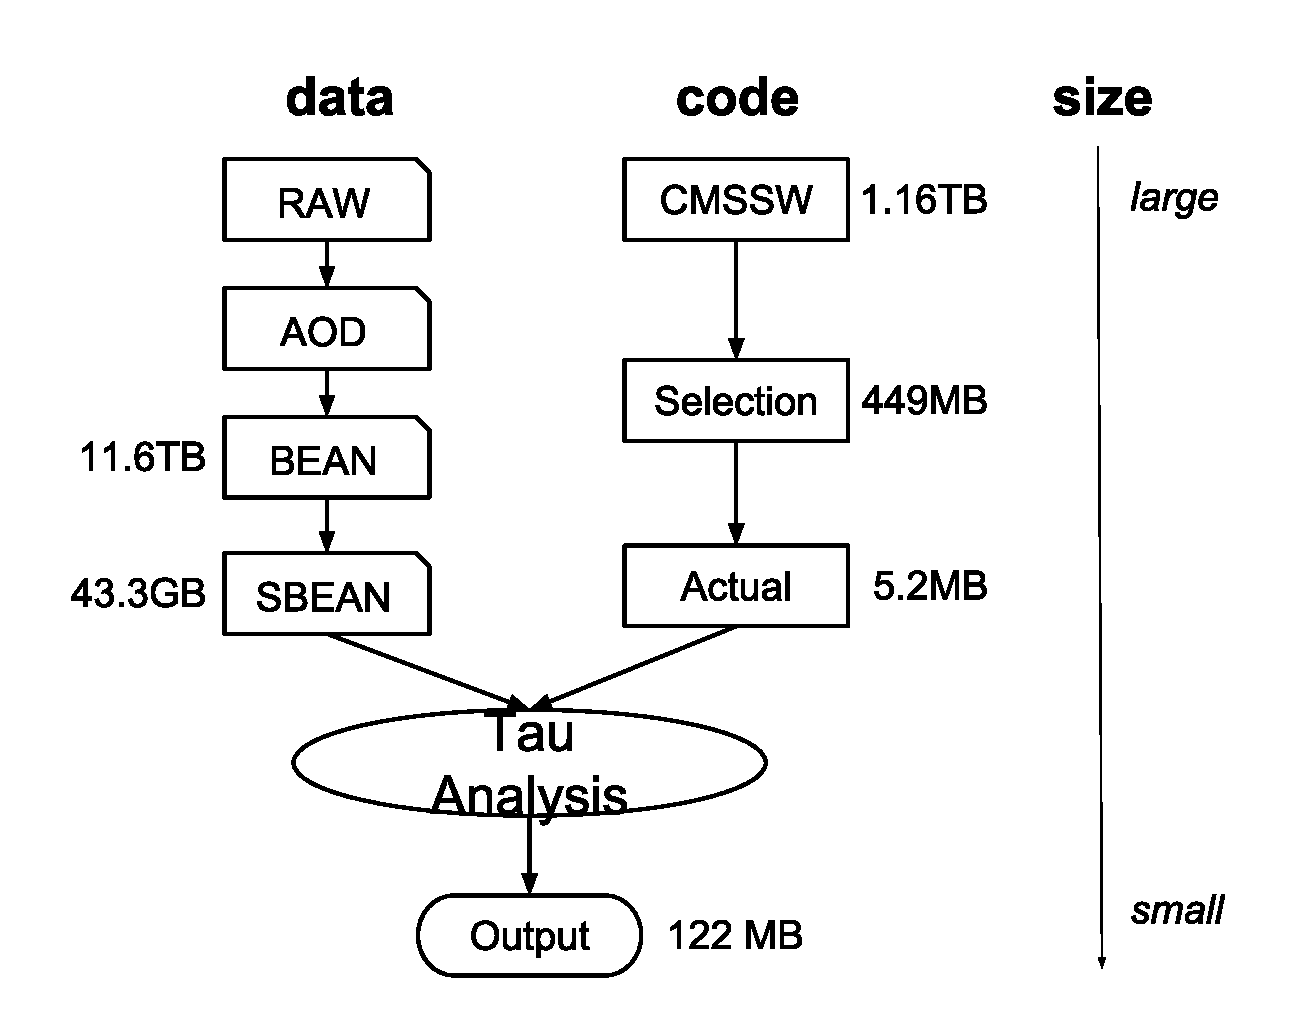
\includegraphics[width=.5\textwidth]{data-code-size.eps}
\caption{Inputs to Tau Roast}
\label{fig:data-code-size}
\end{figure}

\section{Overview of Tau Roast}

The application which is the study of this paper is an CMS application~\cite{collaboration2008cms} called \emph{TauRoast}.
It searches for cases where the Higgs boson decays to two tau leptons~\cite{chatrchyan2013search}.
Since the tau leptons are very short-lived, they are not observed directly, but by the particle decay products 
that they generate.  So, the analysis must search for detector
events that show a signature of decay products compatible with both hadronic tau and top decays.  

Figure~\ref{fig:data-code-size} shows that both the code and data
that form \emph{TauRoast} are drawn from large repositories through
multiple steps of reduction.  A preservation strategy must weigh
whether to store the large repositories completely, the fragments
used by an artifact, or something in between.

{\bf Code Sources.} Like many scientific codes, the central algorithm
of \emph{TauRoast} is expressed in a relatively small amount of
custom code developed by the primary author.  But, the code cannot
run at all without making use of an enormous collection of software
dependencies.  
The largest of these repositories is the CMS Software Distribution (CMSSW)~\cite{cms2006cms},
which contains many different tools, libraries, and utilities.  No single code uses anywhere close to all of these.  But, because it is widely used within the experimental researchers, it is common for users to simply expect that a particular version of the entire repository is available.
 
{\bf Data Sources.}
The CMS collaboration provides end-users with a pre-processed
and reduced data format, AOD~\cite{holtman2001cms}, 
which is based on the RAW output of the CMS detector readout electronics and reconstructed world-wide.
As AOD data are too large to be iteratively processed repetitively in
a physics analysis workflow, it is normally reduced further in
structural complexity and content.  For the analysis under
investigation here, this is a two-step process.  First, the AOD data
are processed at the Notre Dame working group cluster to BEAN (Boson Exploration Analysis Ntuple) events,
containing only trivial data containers packed in vectors.  This step
is time and CPU intensive and its output contains data of 11.6$\,$TB to be
analyzed by the tau analysis.
In the second step, the data are reduced to the ``Ntuple'' format,
which contains only events matching basic quality criteria and
fields relevant to \emph{TauRoast}.
Once the data has been reduced to Ntuples, TauRoast can be run as a single
process, and contains a stringent event selection to look only at high
quality candidate events for the underlying physical process.
Quantities from the relevant events can be
both plotted and used in multivariate analysis to determine the level
of expected signal in real data.


\vspace{-10pt}
\section{Challenges and Observations in Reproducing HEP Applications}

The \emph{TauRoast} and \emph{Athena} application specification was provided to us in the form of an
email which described, in prose, how to obtain the source,
build the program, and run it correctly on one specific
machine at our home institution, with no particular guarantee that
it will run anywhere else in the world. Such level of documentation and exchange of information about a software is typically routine in the scientific world. 
We provide the challenges we faced in capturing the application details in a reproducible form and then preserving it for subsequent reuse:

\begin{itemize}

\item {\bf Identifying all dependencies.}  Due to the distributed nature of HEP applications, the applications typically depend on a large number of external and local dependencies.
External dependencies are often explicitly stated, such as when the application makes connections to Github resources, and CVS servers for downloading source. 
However, when the application has distributed execution then implicit network connections are present requiring us to identify dependencies on all machines where execution takes place. 
Implicit local dependencies arise due to mounted filesystems. In \emph{TauRoast}, the application data and code is distributed on five networked filesystems, and in \emph{Athena} on two networked filesystems. 
Since these filesystems appear local to the application machine, it is important to check and capture mounted filesystems and their respective mount points. 

\item {\bf Configuration Complexity.} To correctly reproduce an application implies that run-time configurations and consistency checks on the available software are effectively captured and preserved. 
For CMS,  {\tt scram} software management tool, is used to locate
the appropriate version of software,  set environment variables such as the PATH, run any
tool-specific configuration, and do the same for all software on which it depends. A reproducible framework must capture the work of such software management tools so that they can conduct similar
checks on a new machine. 

\item {\bf High Selectivity.}  
Although the total size of the resources accessed by HEP
programs is very large, the size of the data and software actually used are much smaller.
Often, an entire repository or data source is named within the script, but the program
only needs a handful of items from that source.  For example, the data is stored on an
HDFS filesystem with 11.6TB of data, but only 18GB are actually consumed by the program. 
Thus there is a size tradeoff of capturing dependencies mentioned in the program and dependencies actually used in the program.
A reproducible framework must include robust rules about not including superfluous dependencies, but including unused dependencies that may potentially get used during program execution.  

\item {\bf Rapid Changes in Dependencies.}  Over the course of three months
between collecting the initial email, analyzing the program, and writing this
paper, the computing environment continuously changed.  The CMSSW software
distribution released a new version, the target execution environment was upgraded
to a new operating system, and the application deprecated the use of CVS for obtaining
the software. In Athena, the computing environment can potentially change daily, since upgrades to the software framework occur on a nightly basis.  
While the users of this software seem be accustomed to constant change,
any preservation technique will have to be very cautious about relying upon an
external service, even one that may appear to be highly stable.

\item {\bf Dependencies for Reproducible Execution.} Capturing the necessary and sufficient dependencies that are part of an application is sufficient for repeatability, but possibly for not reproducibility.
Repeatability implies if a result depends on running program X, we must be able to run exactly X again. In reproducibility the goal is rarely limited to running
\emph{precisely} what a predecessor did. Often, the objective is to
change a parameter or a data input in order to see how the result is affected. To that end, the preservation system must capture enough of the surrounding
material to permit modifications to succeed. 
Further, a better understanding of how end users will consume preserved software will help to shape how
software should be preserved.
\end{itemize}


\vspace{-10pt}
\section{The Invariant Framework}

Given the challenges of reproducing HEP applications, we now describe components of a framework that must be present for other researchers to effectively reproduce the application. 
The framework consists of the following components (also shown in Figure \ref{}:

\begin{itemize}

\item {\bf Capture} In audit phase, PTU captures the execution of the application into a package. The resulting package contains the source code, its dependencies (system files, and files on network such as from CernVM-FS) and the data consumed and written by the application.

\item{\bf Preserve} The generated package is transferred to a Docker container of choice, instantiated from a vanilla, bare-bones image from a particular release (eg., CentOS 6.5, Fedora, or Ubuntu).  The container provides a base execution environment for the package. Now, the container with the package can be saved as a docker image.

\item {Distribute} The saved image can be stored and distributed in a repository like Docker Hub. We imagine these repositories would be preserved, and linked with a digital library.
   
 There are a number of other considerations: is it practical to store the data with the image? What if the �application� requires many processing cores to complete its task? Can one preserve the �DNA� of the application in one small, practical step, yet store everything needed for future reproductions? xHow do we minimize the complexity of the image repository (hub), stemming unnecessary growth and profitably curating the collection?

For purposes of preservation validation, a logical preservation unit (PLU) might be defined which consists of a minimal execution of the software using a small, test data sample, with specified outputs for comparison with future reproduction-validation runs.

A DASPOS preservation testing environment might consist of:

A collection of base images to be used when creating preserved platform-packages
A tool set that assists users in the 1+2+3 steps outlined above
A registry/repo service
A validation service consisting of a number of container slots that can be started on demand
A nightly testing service (Jenkins-like) that continuously monitors the reproducibility state of the preserved application + dependencies + environment + platform.


\end{itemize}


%\section{Evolving the Artifact}
%
%\begin{figure*}[t]
%\centering
%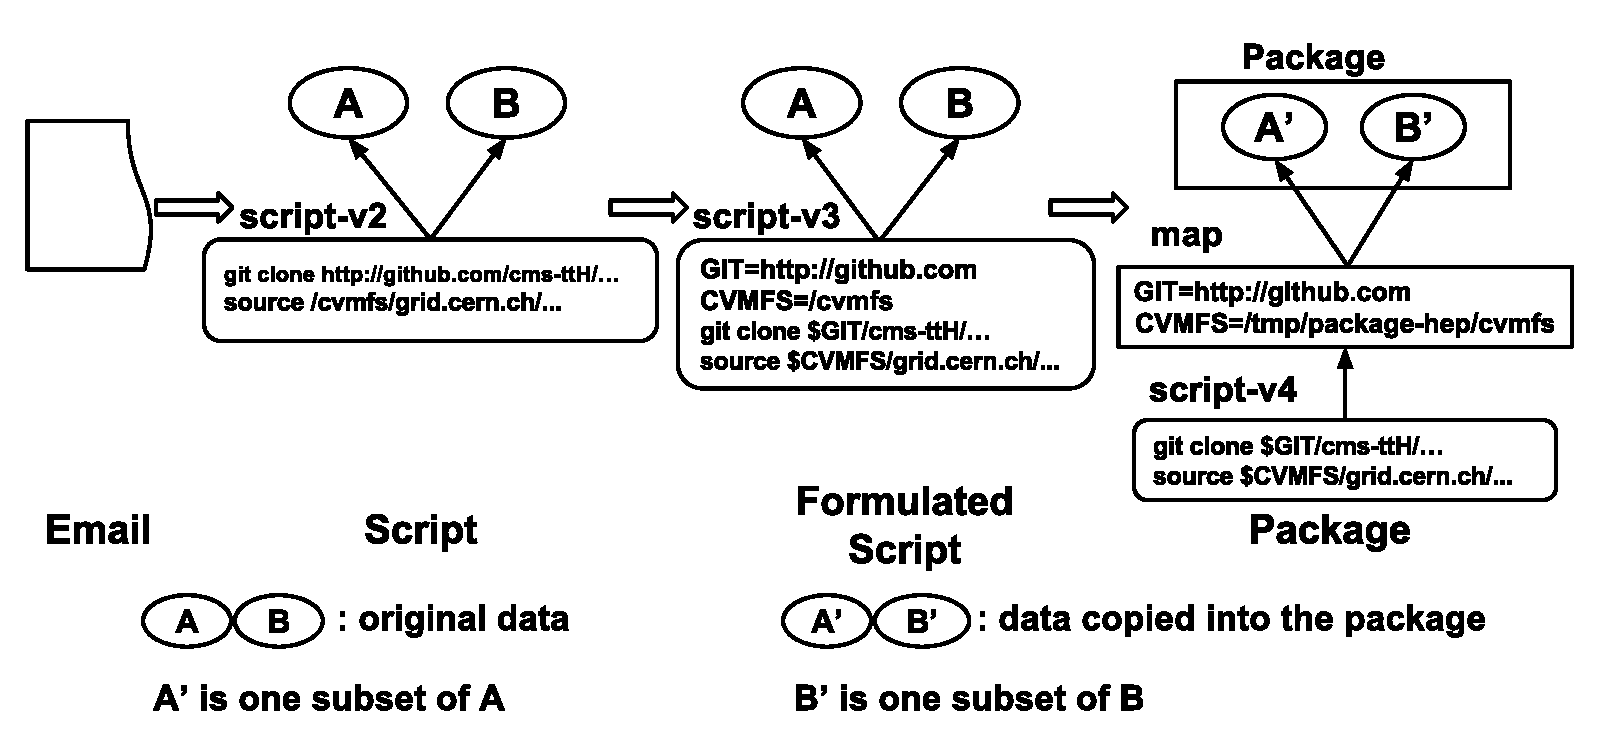
\includegraphics[width=.8\textwidth]{version-evolution.eps}
%\caption{Version Evolution}
%\label{fig:version-evolution}
%\end{figure*}
%
%It is clear that the artifact, as provided, is not in a suitable form
%for preservation.  While it might be technically possible to automatically
%capture the entire virtual machine and all of the connected filesystems,
%it would require 166.8TB of storage, which would be prohibitively expensive
%for capturing this one application alone.  Further, if multiple
%similar applications are preserved, we would miss the opportunity to identify
%common dependencies and store them once for multiple artifacts.
%A more structured approach to dependency management is needed.
%
%Figure~\ref{fig:version-evolution} shows how we have evolved this artifact
%through several stages which make it more suitable for preservation.
%In each step of evolution, we make the dependencies of the artifact
%more explicit and available for analysis and automated processing.
%As noted in the previous section, the original author provided us with
%prose instructions by email which we translated into an
%executable script.  The executable script has embedded in it
%a number of external identifiers such as URLs pointing to repositories
%and paths to networked filesystems.  As a general programming practice,
%embedding such constants into the middle of a program is unwise, and so
%we extract all of those identifiers and place them \emph{outside} the
%script in a \emph{dependency map} or just \emph{map} for short.
%The dependency map lists all of the external dependencies of the application, indicating
%the type, how they are accessed, and where they are currently located.
%The resulting script then simply refers to abstract file locations such
%as \verb$GIT$ and \verb$CVMFS$, while the map file indicates where they
%are currently located. If properly constructed, the script should not refer to any external
%resource unless it is indicated in the dependency map.  We call this idealized
%artifact an \emph{abstract script}.
%
%By extracting the dependencies into the dependency map,
%we introduce great freedom for the curator to move, transform, and otherwise
%manipulate the dependencies of the artifact without damaging the artifact itself.
%A Figure~\ref{fig:version-evolution} shows, it is straightforward for an
%automated tool to examine
%all of the dependencies in the map, download those that are missing,
%and then modify the map to point to the local copies of the dependencies.
%If we group the script, dependency map, and dependencies into a \emph{package},
%we now have a self-contained artifact that can be moved from place to place.
%In some cases, it may be safe to allow the dependency map to refer to 
%trusted remote repositories.  Whether this is advisable is a judgment that
%must be made by the user or the curator, taking into account the long-term
%stability of said repositories.
%
%However, only having the package and the dependency map is not enough. The successful execution of the application on the original machine also relies on the configuration of environment variables.
%We collected the environment variables of the original machine and transformed it into one executable script. If another researcher wants to repeat the application, this executable script will be first executed. 
%The environment variables refer to the dynamic named values defined in the range of one computer, like \verb!$PATH! and \verb!$PYTHONPATH!.
%However, the dependency map refers to the actual storage location of path variables used in one abstract script. For example, the actual storage location of the path variable \verb!CVMFS! 
%is {\tt /data/cvmfs/grid.cern.ch}.
%
%\begin{figure}
%\centering
%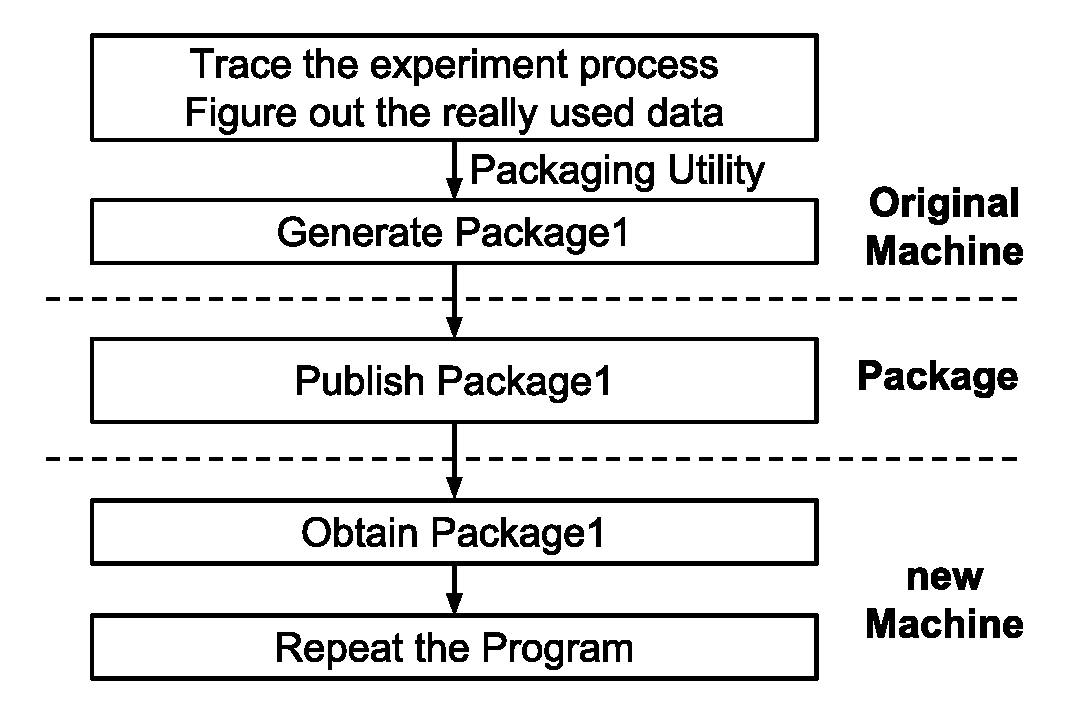
\includegraphics[width=.5\textwidth]{solution3.eps}
%\caption{Relationship of Roles}
%\label{fig:solution3}
%\end{figure}
%
%The relationship of different roles involved in the application preservation and
%reproduction is shown in Figure~\ref{fig:solution3}.  The original author uses the packaging utility to generate the package for one application.
%Then the package, together with
%its map file and description file will be published. When
%another researcher wants to repeat the application, one copy of the package will be downloaded into the new machine and the application can be repeated.
%
%When we try to repeat one application on one new machine, one map file is necessary for the relocation of the data access targets, as
%show in Figure~\ref{fig:version-evolution}. 
%The map file clearly defines the real location of each dependency in the format of dependency variables - the real location of dependency variable {\tt GIT} is \path{/data/git/cms-ttH} and the real location of dependency variable {\tt CVMFS}
%is {\tt /data/cvmfs/grid.cern.ch}.
%The script only refers to the dependency variables defined in the map file.
%This design decouples the application script and the actual data access targets, which minimizes the impact of the evolution of different data dependencies
%and ensures the transparent access.
%The modification of the package only introduces the minimal changes of the map file on the client side.
%
%This basic approach to dependency management is a step in the right direction
%for dependencies that are \emph{explicit} and \emph{external} to the
%user's native execution environment.  However, it leaves two other problems unsolved.
%
%First, the basic approach requires that someone be \emph{aware} of the dependencies,
%whether it be the end user, the system administrator, or the archive curator.
%It seems reasonable to expect the user to be aware of a large dependency mentioned in a top-level script.
%But, oftentimes the dependency is embedded invisibly deep within the software stack,
%or is connected to the machine by the local system administrators.  No single party
%is likely to have complete information about all of the dependencies.
%Second, the basic approach assumes that the entire dependency is actually
%consumed by the artifact.  As we have suggested above (and will show below),
%this sort of program often only consumes a small fraction of what it does declare
%as a dependency.
%
%To address both of these problems, users and curators alike need tools that
%will automatically observe the dependencies of complex applications, to
%facilitate automatic and efficient preservation.
%

\vspace{-10pt}
\section{Component Tools for Reproducible Research}

We have constructed a first approximation of the invariant framework
by using and modifying a variety of existing technologies.  Of course,
a viable long-term strategy for reproducibility must not depend on a single
technology.
To this end, we have identified several technologies and techniques
that can implement each stage of the framework.

{\bf Capturing Dependencies.}  The Unix {\tt ptrace} mechanism
allows a tracing process to observe all of the system calls performed by
an application, inferring each of the resources upon which an application
depends.  We have extended two existing tracing tools in order to capture
dependency information at the granularity of files and directories. 
Dependency may refer to source code, if available, or a binary.

Parrot~\cite{thain2005parrot} is a virtual filesystem access tool which
is used to attach applications to a variety of remote I/O systems such as HTTP, FTP, and CVMFS. It works by trapping system calls through the {\tt ptrace} interface,
replacing selected operations with remote accesses.  As a side-effect, Parrot is
also able to modify the filesystem namespace in arbitrary ways according to user
needs.  Parrot is particularly used in the high energy physics community
to provide remote access to application software.
To capture dependencies, we made small modifications to Parrot to record
the logical name of every file accessed by an application into an external
dependency list.  After execution is complete, a second tool is used to copy
all of the named dependencies into a package.

PTU~\cite{PTU,pham2014framework} is designed to create a package of an application by recording all of the binaries, libraries, scripts, data files, and environment variables used by a program.   PTU uses the CDE~\cite{guo2011cde} technology to observe system calls, but takes a snapshot of every file at the point of access.  In addition to files, PTU records \emph{metadata} about the execution environment, such as kernel versions, application versions, and dynamic library versions by using standard Unix commands.  PTU also records \emph{provenance} in the form of a graph that describes how each file is created or consumed by processes within the application.  Because PTU is focused solely on the problem of preservation, it can achieve lower overhead than Parrot when remote data access is not a requirement, as we show below.

{\bf Preservation of Dependencies.}  Both Parrot and PTU can observe the precise
set of files accessed by an application.  If this precise list of files is preserved
then it should be possible to execute
\emph{exactly} the same application on \emph{exactly} the same inputs a second
time.  However, if the objective is to \emph{re-purpose} the application by running it in slightly different configurations, then the preserved package may need to
be more comprehensive than the strict dependency list.

There are many possible heuristics for creating the preserved package
from the dependency list.  We have implemented three:
In a {\bf shallow copy}, we simply copy only
the exact dependencies.  Where a directory was listed, a directory is created and populated with empty files as placeholders to facilitate a directory listing.  In a {\bf medium copy},every file in every directory mentioned by the application is preserved one level deep.  In a {\bf deep copy}, every file in every directory mentioned by the application is copied recursively.  Obviously, the more aggressive the preservation, the larger the package, but the greater possibility that it can be adapted to other uses.  Other approaches to package generation might including generating the union
of multiple dependency sets, or allowing the expert user to manually add
and remove dependencies.

Both Parrot and PTU generate packages that consist of plain filesystem trees representing the namespace and data of the preserved application, and can be easily transformed into whatever archive format (e.g. ZIP or TGZ) is most suitable.  This is desirable for long-term preservation that may outlive various deployment technologies.
However, neither technology yet integrates the programming environment envisioned above for the documentation purpose.  Without these techniques, the preserved packages will have diminishing value over time.

{\bf Distribution and Deployment.}
Once generated, application packages must be collected, curated, and made
available through publically shared repositories.  There currently exist a
wide variety of services and efforts to share binary objects in this way,
and so we assume such a service will be available in the future.

Of more immediate interest is the ability to deploy a preserved
package at a desired execution site.  Again, long-term preservation
requires artifacts that are independent of any particular technology,
so the package must be sufficiently self-describing
to work with multiple technologies.  The packages produced by both Parrot and PTU
can today be re-executed through any of the following mechanisms:

(1) Re-running the application through Parrot, which can dynamically construct
the desired namespace and limit file accesses to within the preserved package.
(2) Generating a virtual machine image from the package, which can be loaded
into a local virtual machine monitor, or transferred to a cloud service provider.
(3) Converting the package into a Docker image format, enabling it to be
deployed within a lightweight Linux container.

 % Docker images
\vspace{5pt}
\noindent{\bf Linux Containers and Docker Images:} Linux Containers provide multiple isolated execution instances on top of the same kernel through OS-level virtualization. Thus they can be used to persist the captured packages into images. 
Using such containers, Docker now allows to preserve the image in a more user-friendly way. 
Docker also provides portable deployment of containers across platforms, documentation of packages in a scriptable format, and versioning of container images. The image can be preserved along with dockerfiles, which are text files that contain all the commands to build a Docker image: the computational part is similar to shell scripts and can help provision similar to other provisioning tools (e.g. Chef, Puppet) and the text part is for human consumption and more suited for use with a version management system such as subversion or git, which can track any changes made to the Dockerfile. Thus dockerfiles can be used to preserve the namelist of Parrot packages and provenance description in PTU. 
Docker is integrated with a continuous build environment which will check and validate the version of the software being used, and use a more recent version to build application software. 

\begin{figure*}
\centering
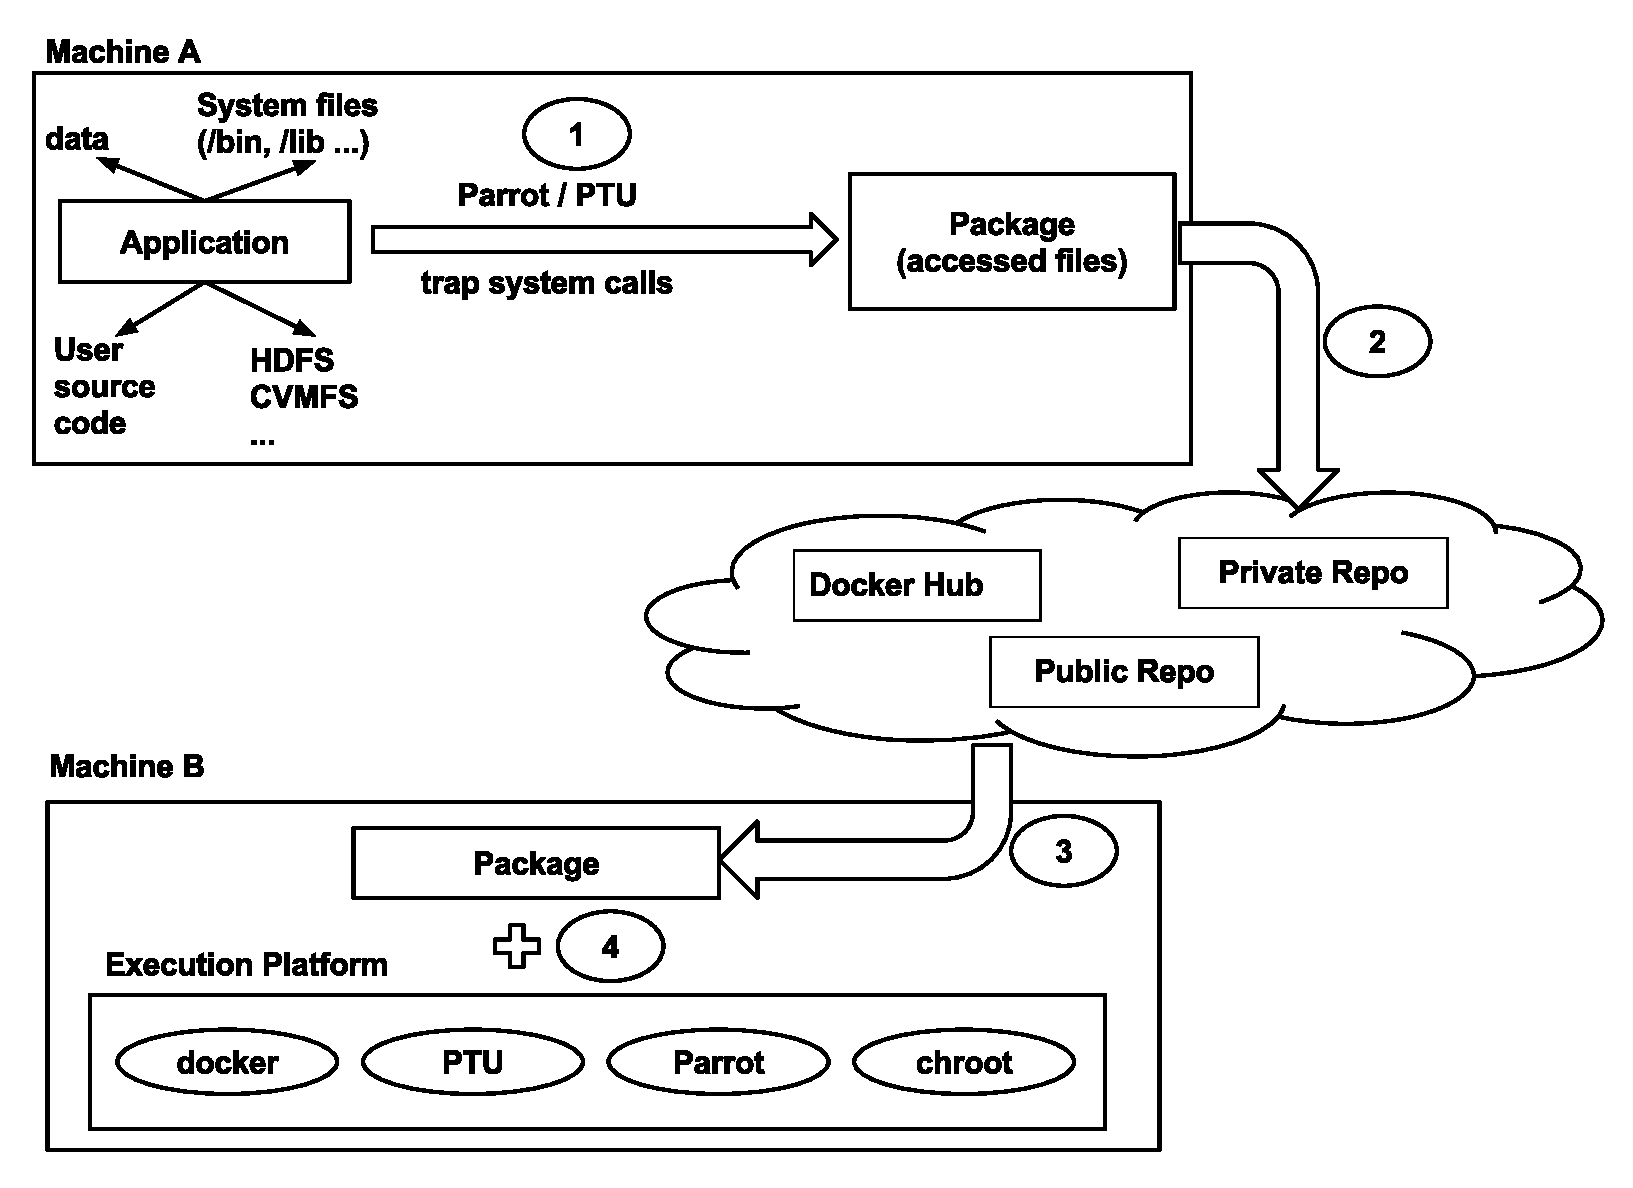
\includegraphics[width=1.0\textwidth]{preservation_framework.eps}
\caption{Preservation Framework}
\label{fig: preservation_framework}
\end{figure*}


\vspace{-10pt}
\section{Evaluation}

We evaluated the correctness and performance of running, packaging, and re-running the Athena and TauRoast application using Parrot and PTU.
To do this, the application was first executed directly, its execution time and output were recorded. Then the application was executed under Parrot and PTU, and a self-contained package was created for each case. Finally, the application was re-executed using the package. The time overhead of each execution and re-execution was collected and compared with the recorded reference.

The TauRoast application checks and evaluates a dataset with the size of 18 GB stored in HDFS, and can be finished in about 20 minutes when running directly on a server with 64 cores and 126 GB memory. The output of the application includes an event analysis log and a statistics information, and its size is 289 KB. The Athena application processes a given input data file to produce four derived data files. It uses the nightly release of the Athena framework and 
submits an analysis job to obtain derived data.  

\begin{table}
\small
    \centering
    \begin{tabular}{lcccc}
    \hline
    \bf Application & \bf Tool Type & \bf Obtain Namelist & \bf Create Package & \bf Re-Execution \\ \hline
	Athena & Parrot & 10 min 14 sec & 53 sec & 9 min 14 sec \\ \hline
	Athena & PTU & --- & 8min 48 sec & 7 min 21 sec \\ \hline
	TauRoast & Parrot & 22 min 50 sec  & 4 min 25 sec & 10 min 24 sec \\ \hline
	TauRoast & PTU & --- & 23 min 30 sec & 8 min 40 sec \\ \hline 
    \end{tabular}
    \normalsize
    \caption{Time Comparison between Parrot and PTU}
    \label{table:parrot_ptu}
\end{table}    

Table~\ref{table:parrot_ptu} compares the time overhead of preserving Athena and TauRoast application using Parrot and PTU.
Parrot splits the packaging creation procedure into two sequential steps: first, execute the application within Parrot and generate the accessed file namelist; second, traverse the namelist and copy all the accessed files into a self-contained package.
PTU accomplishes the execution procedure and the package creation procedure concurrently through multi-threading, bringing 17.5\% additional time overhead.

The re-execution time is half or less than half of the original execution time in both cases of the \emph{TauRoast} application. During the original execution, the input dataset is either locally available or comes from HDFS, which is accessed through FUSE. During the package creation procedure, all the input dataset has been copied from HDFS into the package on the local filesystem. So, the re-execution procedure can get its input from the local filesystem instead of obtaining the input dataset from HDFS.

Both packages created by Parrot and PTU are a subset of the root filesystem, which only includes all the accessed files. The original relationship, such as symbolic links, between files and directories is maintained. The files from pseudo filesystems such as proc and dev, are ignored. The re-execution procedure uses these pseudo filesystems from the host machine through redirection techniques.
For the \emph{TauRoast} application, the sizes of the packages created by Parrot and PTU are nearly the same, 18GB. 
Except for the accessed files, both Parrot and PTU preserve the execution environment of the application. 
the PTU package also includes a leveldb-format provenance information of the application with the size of 3 MB.

\begin{table}
\small
	\centering
	    \begin{tabular}{lcrr}
	        \hline
	        \bf Dependency Name & \bf Location & \bf Total Size &  \bf Used Size\\ 
	        \hline
	        CMSSW code     & CVS & 88.1GB &  5.2MB\\ \hline
	        Tau source       & Git & 73.7MB & 212KB \\ \hline
	        PyYAML binaries    & HTTP & 52MB& 0KB \\ \hline
	        .h file       & HTTP& 41KB & 0KB \\ \hline 
	        Ntuples data    & HDFS& 11.6TB & 18GB \\ \hline
	        Configuration & CVMFS & 7.4GB & 105MB \\ \hline
	        Linux commands & localFS & 110GB & 110MB \\ \hline     
	        HOME dir& AFS &12GB & 24MB\\ \hline
	        Misc commands & PanFS & 155TB & 8KB \\ \hline
	        Total      &    & 166.8TB     &  18GB \\ \hline
	    \end{tabular}
	    \normalsize
	    \caption{Data and Code Size Used by TauRoast}
	    \label{table:size-original-real}
\end{table}
%	\begin{tablenotes}
%	      \small
%	      \item The first column illustrates the total size of each data and software source; 
%	            the second column illustrates the size of the named files from each source;
%	            the third column illustrates the size of actually used data from each source.
%	            N/A denotes it is hard to figure out the named size of implicit dependencies directly.        
%	    \end{tablenotes}
	   
Table~\ref{table:size-original-real} illustrates the total size and actually used size of each source for TauRoast. 
The total size is too large to be put into a separate image. However, the actually used size is greatly reduced to be 18 GB.
Within the package, the input dataset nearly occupies the whole package. All the other libraries and software dependencies only occupies about 200 MB.
As the input dataset grows, it can be put outside the package to reduce the shipping time of the package.

In Athena, the input file is 224MB and output files are 16MB. PTU build a 855MB package, while Parrot builds an 825MB package. The overhead is of provenance which is 7MB and 
some differences is dependency information. 

\vspace{-10pt}
\section{Related Work}

%Generally, there are three approaches to preserve a software environment:
%hardware preservation, migration and emulation.  Hardware
%preservation preserves the original software and its original operating
%environment. 
%Software migration technique~\cite{cifuentes1996binary,mancl2001refactoring} is used to facilitate running software on new machines.
%However, migration often involves the re-compiling and re-configuring
%the source code to accommodate a new hardware platform and software environment.
%Emulation recreates the original software and hardware environment by
%programming future platforms and OSs. Virtual machine is one common way to implement this. According to the usage and degree of emulation of the real
%machine, virtual machine can be divided into system virtual machine and process
%virtual machine. The working and design principles and
%performance evaluation of system virtual machine were illustrated in~\cite{goldberg1974survey, smith2005architecture}. 
%Further, the functionality of system VM to support different guest operating systems was illustrated in~\cite{barham2003xen,kivity2007kvm,rosenblum1999vmware}.
%%F. Esquembre~\cite{esquembre2004easy} illustrated how JVM, one process virtual machine, can expedite the creation of
%%scientific simulations in Java. 
%The pros and cons of these three approaches were discussed in~\cite{matthews2009towards,phelps2005no,hong2010software}.

The capture and preserve environments were treated as one entity in~\cite{matthews2009towards,phelps2005no,hong2010software}. 
However, frequently changing experiment software makes the maintenance of the captured experimental environment very complex. 
CernVM~\cite{buncic2010cernvm} treated them as two different categories. 
The capturing of computing environment is implemented within CernVM, and the preservation of software environment is based on a CernVM filesystem(CVMFS) specifically designed for efficient software distribution.
In fact CVMFS~\cite{buncic2010cernvm} published pre-built and configured experiment software releases to avoid the time-consuming software building procedure, i.e, it did not 
preserve software in source code format as emphasized in~\cite{zabolitzky2002preserving,castagne2013consider}. 
However, as we show a simple VMI of binaries can also be too big in size for distribution, and the preservation itself needs to include a documentation stage and a distribution stage. 
We have described capture tools that include software code when available to be included in the package. 

%Current mechanisms of preserving scientific experiments assume that all the data and software mentioned in the experiments are necessary for the reproduction of the experiments. 
%However, this is not always the case. In some cases, the original author may leave additional code referring to irrelative data and software in the application or the application may require additional 
%data and software for reproducibility. 

%One mechanism, which can figure out the absolutely relevant data and software of one experiment, is important for both the preservation and reproduction of scientific experiments.

Attempts from different perspectives to facilitate the reproduction of scientific experiments utilizing a preserved software library have been made. 
The software distribution mechanism over network was discussed in~\cite{compostella2010cdf, blomer2011cernvm}.
J. R. Rice et al.~\cite{rice1996scientific} describe a distribution hub through the integration of user interface, scientific software libraries, knowledge base into problem-solving environment.
S. R. Kohn et al.~\cite{kohn2001divorcing} tried to enable the creation and distribution of language-independent software library by addressing language interoperability.
a scalable, distributed and dynamic workflow system for digitization processes was proposed in~\cite{schoneberg2013scalable}.
A distributed archival network was designed in~\cite{subotic2013distributed} to facilitate process-oriented automatic long-term digital preservation.
M. Agosti et al.~\cite{agosti2012envisage} aimed to help non-domain users to utilize the digital archive system developed for domain experts.

B. Matthews et al.~\cite{matthews2008significant} introduced one conceptual framework for software preservation from several case studies of software preservation.
One tool to capture software preservation properties within a software environment was designed in~\cite{matthews2010framework} through a series of case studies conducted to evaluate the software preservation framework.
L. R. Johnston et al.~\cite{johnston2014workflow} proposed one overall data curation workflow for 3-5 case studies of preserving research data.
Two case studies~\cite{borgman2012data} were conducted to figure out the properties of data to be reused in the future.




%Generally, there are three approaches to preserve a software environment:
%hardware preservation, migration and emulation.  Hardware
%preservation preserves the original software and its original operating
%environment. 
%Software migration technique~\cite{cifuentes1996binary,mancl2001refactoring} is used to facilitate running software on new machines.
%However, migration often involves the re-compiling and re-configuring
%the source code to accommodate a new hardware platform and software environment.
%Emulation recreates the original software and hardware environment by
%programming future platforms and OSs. Virtual machine is one common way to implement this. According to the usage and degree of emulation of the real
%machine, virtual machine can be divided into system virtual machine and process
%virtual machine. The working and design principles and
%performance evaluation of system virtual machine were illustrated in~\cite{goldberg1974survey, smith2005architecture}. 
%Further, the functionality of system VM to support different guest operating systems was illustrated in~\cite{barham2003xen,kivity2007kvm,rosenblum1999vmware}.
%%F. Esquembre~\cite{esquembre2004easy} illustrated how JVM, one process virtual machine, can expedite the creation of
%%scientific simulations in Java. 
%The pros and cons of these three approaches were discussed in~\cite{matthews2009towards,phelps2005no,hong2010software}.
%
%The preservation of computing environment and software environment was treated as one entirety in~\cite{matthews2009towards,phelps2005no,hong2010software}. 
%However, frequently changing experiment software makes the maintenance of the preserved experimental environment very complex. 
%CernVM~\cite{buncic2010cernvm} treated them as two different categories. 
%The preservation of computing environment is implemented with CernVM, and the preservation of software environment is based on a CernVM filesystem(CVMFS) specifically designed for efficient software distribution.
%In our work, we have distinguished between capture and preserve phases but extended to include automated mechanisms. 
%
%The importance of preserving software in source code format was emphasized in~\cite{zabolitzky2002preserving,castagne2013consider}. 
%However, CVMFS~\cite{buncic2010cernvm} published pre-built and configured experiment software releases to avoid the time-consuming software building procedure. 
%
%Attempts from different perspectives to facilitate the reproduction of scientific experiments utilizing a preserved software library have been made. 
%The software distribution mechanism over network was discussed in~\cite{compostella2010cdf, blomer2011cernvm}.
%J. R. Rice et al.~\cite{rice1996scientific} made the reproduction process easier through the integration of user interface, scientific software libraries, knowledge base into problem-solving environment.
%S. R. Kohn et al.~\cite{kohn2001divorcing} tried to enable the creation and distribution of language-independent software library by addressing language interoperability.
%a scalable, distributed and dynamic workflow system for digitization processes was proposed in~\cite{schoneberg2013scalable}.
%A distributed archival network was designed in~\cite{subotic2013distributed} to facilitate process-oriented automatic long-term digital preservation.
%M. Agosti et al.~\cite{agosti2012envisage} aimed to help non-domain users to utilize the digital archive system developed for domain experts.
%
%Current mechanisms of preserving scientific experiments assume that all the data and software mentioned in the experiments are necessary for the reproduction of the experiments. However, this is not always right. In some cases, the original author may leave additional code referring to irrelative data and software in the program. One mechanism, which can figure out the absolutely relevant data and software of one experiment, is important for both the preservation and reproduction of scientific experiments.
%
%B. Matthews et al.~\cite{matthews2008significant} introduced one conceptual framework for software preservation from several case studies of software preservation.
%One tool to capture software preservation properties within a software environment was designed in~\cite{matthews2010framework} through a series of case studies conducted to evaluate the software preservation framework.
%L. R. Johnston et al.~\cite{johnston2014workflow} proposed one overall data curation workflow for 3-5 case studies of preserving research data.
%Two case studies~\cite{borgman2012data} were conducted to figure out the properties of data to be reused in the future.
%

\vspace{-10pt}
\section{Conclusions and Future work}
In this paper, we propose an invariant framework for conducting reproducible computational science - using light-weight virtualization approaches to preserve applications in the format of self-contained packages and using standardized software delivery mechanisms to deliver and distribute preserved packages.
We use two complex high energy physics applications to illustrate how the framework can help the original authors preserve and distribute the applications, and others reproduce the applications.
This paper focuses on how to measure the mess and track the used dependencies to preserve an application.
In the following work, we plan to explore how to preserve an application in an organized style - specifying the execution environment clearly.
How to preserve and improve the availability of remote network resources is another important problem to be explored.

\small
\vspace{-10pt}
DOI for the experiment involved in the paper: \url{doi:10.7274/R0C24TCG}

\section*{Acknowledgments}

This work was supported in part by National Science Foundation grants PHY-1247316 (DASPOS), 
OCI-1148330 (SI2), PHY-1312842, ICER-1440327, SES-0951576 (RDCEP), and ICER-1343816 (UChicago subcontract).
The University of Notre Dame Center for Research Computing scientists and engineers provided critical technical assistance throughout this research effort.
The Open Science Grid at the University of Chicago provided critical technical assistance throughout this research effort.

\vspace{-10pt}
\bibliographystyle{plain}
\bibliography{cclpapers,this,sole}

\end{document}
